\documentclass[conference]{IEEEtran}
\usepackage{graphicx}
\usepackage{booktabs}
\usepackage{amsmath,amssymb}
\usepackage{fontspec}
\setmainfont{texgyretermes}[Extension=.otf, UprightFont=*-regular, BoldFont=*-bold, ItalicFont=*-italic, BoldItalicFont=*-bolditalic]
\usepackage{cite}
\usepackage{url}
\graphicspath{{../docs/diagrams/}{../results/}}

\begin{document}

\title{A TPU-Inspired Output-Stationary Systolic Array\\for 8-bit Matrix Multiplication in Verilog}

\author{
\IEEEauthorblockN{Vetriselvan R, Hrishi Dongre, Pampana Sree Adithya, Ishan Goyal, Vedant Madne}
\IEEEauthorblockA{Team PowerPuffBoys, Section A\\
Modern Computer Architecture, B.Tech CS\&AI\\
Phase I Report}
}

\maketitle

\begin{abstract}
Matrix multiplication dominates the computation in neural network inference. This report presents the Phase I design of a small systolic-array accelerator, in the style of the matrix unit of Google's Tensor Processing Unit, written in synthesizable Verilog-2001. The design uses an output-stationary dataflow: each of the 16 processing elements (PEs) of a 4$\times$4 grid multiplies signed 8-bit operands and keeps its own 32-bit accumulator, while operands move one PE per clock cycle. Input staggering (skew) is done in hardware with per-row and per-column delay lines, and a four-state controller sequences each run. The design is parameterized in array size $N$ and inner dimension $K$. It was verified in Icarus Verilog against a NumPy reference model on 106 matrix pairs per configuration, including directed edge cases, for $N \in \{2,3,4,8\}$. A $4\times4\times4$ product completes in 12 cycles against 65 cycles for a sequential single-MAC baseline (5.4$\times$), and the speed-up rises to 14.2$\times$ at $K=64$, approaching the 16$\times$ limit. Yosys synthesis for a Xilinx 7-series target maps the 4$\times$4 array onto 16 DSP slices.
\end{abstract}

\section{Introduction}
Fully connected and convolutional layers reduce to general matrix multiplication, so hardware that multiplies matrices efficiently speeds up most of a neural network. Running $C = AB$ for $A \in \mathbb{Z}^{M\times K}$ and $B \in \mathbb{Z}^{K\times N}$ needs $MNK$ multiply-accumulate (MAC) operations. A processor with one MAC unit needs about $MNK$ cycles; a grid of $M \times N$ MAC units can, in principle, do $MN$ MACs per cycle.

The difficulty is feeding the grid. If every unit fetched its operands from memory, memory bandwidth would limit the design. A systolic array avoids this: each operand enters at the edge of the grid and is passed from neighbour to neighbour, so one memory read is reused by a whole row or column of PEs.

This project, Project 12 of the course, builds such an array in Verilog, verifies it in simulation, and compares it with a sequential baseline. Phase I covers the complete working design, its verification, and first performance and synthesis results.

\section{Literature Review}
\textbf{Systolic arrays.} Kung~\cite{kung1982} introduced systolic architectures as a general method for mapping regular computations onto hardware: data flows rhythmically from memory through a network of simple cells that communicate only with neighbours, so each value fetched is used many times. Linear and two-dimensional (rectangular, triangular, hexagonal) arrays were described.

\textbf{The Tensor Processing Unit.} Jouppi et al.~\cite{jouppi2017} evaluated Google's first TPU, an inference chip deployed in datacenters since 2015. Its core is a matrix unit of 65,536 8-bit MACs giving a peak of 92 TOPS, and it was on average 15--30$\times$ faster than contemporary CPUs and GPUs on production MLP, CNN and LSTM workloads, with 30--80$\times$ better performance per watt. Its success with low-precision MACs in a systolic grid motivates our choice of 8-bit operands.

\textbf{Dataflows.} Chen et al.~\cite{chen2016} classified accelerators by which data each PE reuses locally: weight-stationary (WS), output-stationary (OS), no local reuse, and their row-stationary scheme. SCALE-Sim~\cite{samajdar2018} gives cycle-level models for OS, WS and input-stationary arrays; in OS, each output is pinned to a PE while inputs stream from the left and weights from the top, and reduction happens in place. Gemmini~\cite{genc2021} supports both OS and WS in one generator and notes that WS needs an accumulator outside the array.

\textbf{Integer arithmetic.} Jacob et al.~\cite{jacob2018} showed that neural networks can run inference with 8-bit weights and activations and 32-bit accumulators, close to floating-point accuracy, which justifies the int8/int32 widths used here.

\section{Proposed Solution}

\subsection{Overall architecture}
Fig.~\ref{fig:block} shows the top-level module \texttt{mm\_accel}. A write port loads matrices $A$ and $B$ into on-chip buffers. When \texttt{start} is raised, the controller clears all accumulators and then steps a cycle counter $t$. While $t < K$, the feeders present column $t$ of $A$ (one value per row) and row $t$ of $B$ (one value per column). Two skew blocks delay row $i$ by $i$ cycles and column $j$ by $j$ cycles before the values enter the PE grid. When the last product is accumulated, the controller raises \texttt{done} and the 16 results are read in parallel.

\begin{figure*}[t]
\centering
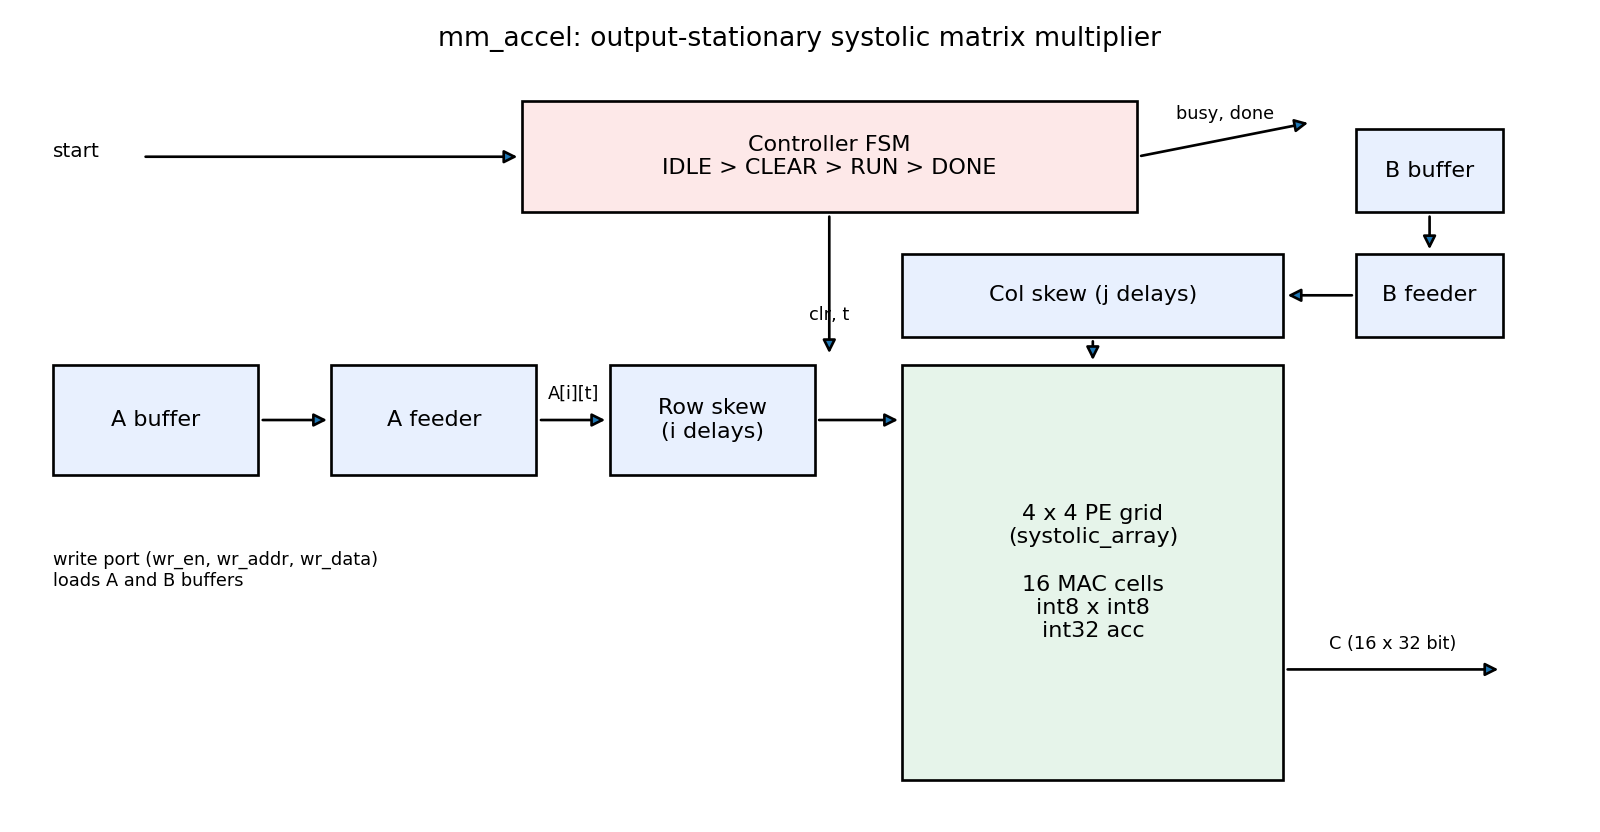
\includegraphics[width=0.85\textwidth]{block_diagram.png}
\caption{Block diagram of the accelerator.}
\label{fig:block}
\end{figure*}

\subsection{Processing element}
Each PE (Fig.~\ref{fig:pe}) multiplies its two signed 8-bit inputs, adds the product to a signed 32-bit accumulator, and forwards $a$ to the right and $b$ downward through registers, so each hop costs one cycle. A synchronous \texttt{clr} input zeroes the accumulator between runs. The product of two int8 values lies in $[-16256, 16384]$, so a sum of $K$ products needs at most $16 + \lceil\log_2 K\rceil$ bits; 32 bits are safe for $K$ up to 131,071.

\begin{figure}[t]
\centering
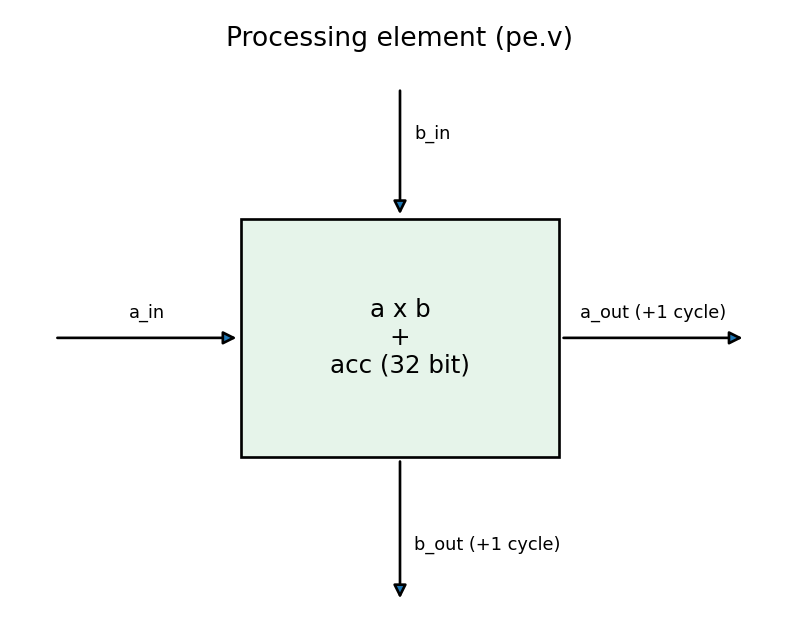
\includegraphics[width=0.62\columnwidth]{pe.png}
\caption{Processing element: one MAC with pass-through registers.}
\label{fig:pe}
\end{figure}

\subsection{Output-stationary dataflow and skew}
We chose OS because every result stays in its PE: no weight-loading phase, no partial sums moving between PEs, and no adders outside the array. With row $i$ delayed by $i$ cycles and column $j$ by $j$, PE$(i,j)$ receives $A[i][k]$ and $B[k][j]$ with the same index $k = t - i - j$ at cycle $t$, which produces the diagonal wavefront of Fig.~\ref{fig:wave}. The last PE finishes at $t = M + N + K - 3$, so the compute phase takes
\begin{equation}
T_{\text{sys}} = M + N + K - 2 \text{ cycles,}
\end{equation}
compared with $T_{\text{seq}} = MNK$ for one MAC unit. Each skew lane is a shift register of $i$ byte-wide stages; the feeders drive zeros outside the valid window so idle PEs add zero.

\begin{figure*}[t]
\centering
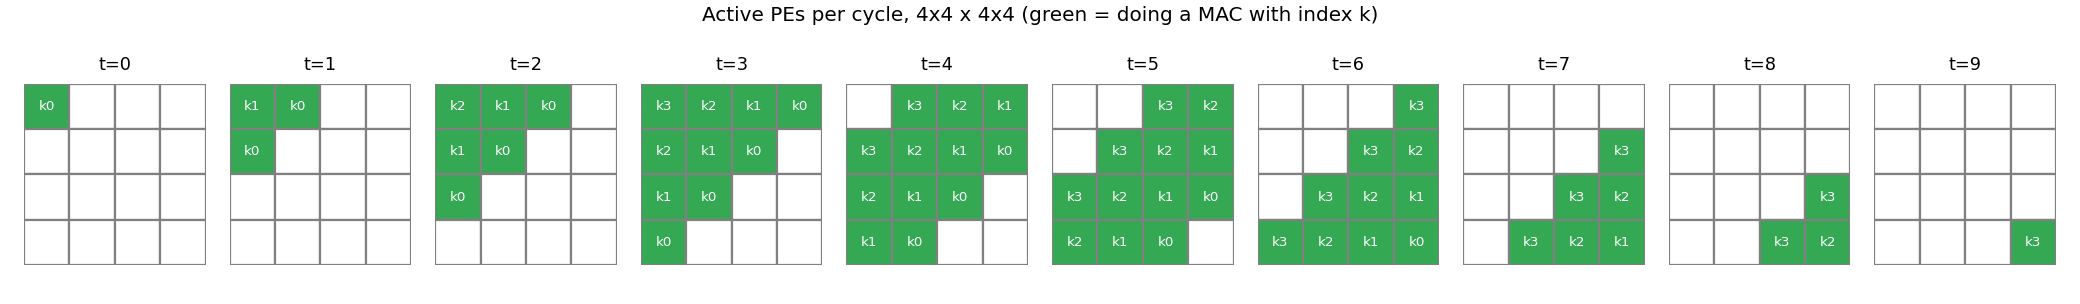
\includegraphics[width=\textwidth]{wavefront.png}
\caption{Active PEs per cycle for a $4\times4\times4$ product. Each green cell performs the MAC with index $k$.}
\label{fig:wave}
\end{figure*}

\subsection{Controller}
The controller is a four-state Moore machine: IDLE waits for \texttt{start}; CLEAR pulses \texttt{clr} for one cycle; RUN increments $t$ from 0 to $2N + K - 3$; DONE holds the results and asserts \texttt{done}. A new \texttt{start} in DONE begins the next run.

\subsection{Verification}
A Python script generates test cases and expected results with NumPy and writes them as two's-complement hex files read by the Verilog testbench through \texttt{\$readmemh}. Each configuration runs 6 directed cases (identity, all zeros, all $-128$, alternating $127/-128$, a single non-zero element, non-symmetric matrices) and 100 random cases. Separate unit testbenches check the PE (including $-128 \times -128$ and the clear signal), the skew delays, and a bare 2$\times$2 array driven with hand-computed skewed inputs. A cycle-level Python model of the array confirmed the timing formula against NumPy on 200 random shapes. To check that the testbench detects faults, three bugs were injected (controller finishing one cycle early, missing skew, unsigned multiply); each produced failures.

\subsection{Baseline}
The baseline \texttt{seq\_mac} has the same interface and buffers but a single MAC unit stepping through $i$, $j$ and $k$, one MAC per cycle.

\section{Preliminary Results}
Both designs passed all 106 cases for each of the configurations $(N,K) = (2,2), (3,3), (4,4), (4,16)$ and $(8,8)$. Table~\ref{tab:perf} lists measured cycles from \texttt{start} to \texttt{done}. The array always takes $T_{\text{sys}} + 2$ cycles (one to sample \texttt{start}, one to clear) and the baseline $MNK + 1$. Fig.~\ref{fig:speed} shows that as $K$ grows, fill and drain matter less and the speed-up approaches the 16$\times$ limit set by the number of PEs.

\begin{table}[t]
\centering
\caption{Measured latency (cycles) and speed-up}
\label{tab:perf}
\begin{tabular}{rrrrrr}
\toprule
$N$ & $K$ & Model & Systolic & Sequential & Speed-up \\
\midrule
2 & 2 & 4 & 6 & 9 & 1.50 \\
3 & 3 & 7 & 9 & 28 & 3.11 \\
4 & 4 & 10 & 12 & 65 & 5.42 \\
8 & 8 & 22 & 24 & 513 & 21.38 \\
4 & 16 & 22 & 24 & 257 & 10.71 \\
4 & 64 & 70 & 72 & 1025 & 14.24 \\
\bottomrule
\end{tabular}
\end{table}

\begin{figure}[t]
\centering
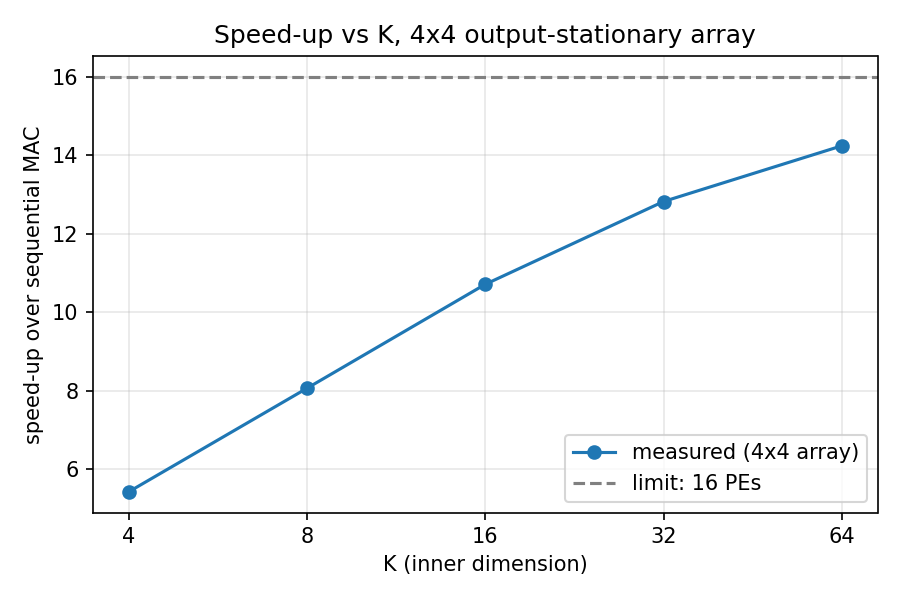
\includegraphics[width=\columnwidth]{speedup_vs_k.png}
\caption{Speed-up over the sequential baseline for a 4$\times$4 array as $K$ grows.}
\label{fig:speed}
\end{figure}

Table~\ref{tab:synth} gives Yosys 0.70 synthesis results for a Xilinx 7-series target (\texttt{synth\_xilinx}). Each PE maps to one DSP48E1 slice. Yosys does not provide a reliable maximum frequency without place-and-route timing data; fmax will be obtained with Vivado in Phase II. The results bus is fully parallel ($32N^2$ output bits), which suits simulation; a board version would read results through a narrower port.

\begin{table}[t]
\centering
\caption{Yosys synthesis results (Xilinx 7-series)}
\label{tab:synth}
\begin{tabular}{lrrrr}
\toprule
Design & DSP48E1 & LUTs & RAM prim. & FFs \\
\midrule
Systolic $2\times2$ & 4 & 68 & 0 & 94 \\
Systolic $4\times4$ & 16 & 75 & 16 & 176 \\
Systolic $8\times8$ & 64 & 142 & 48 & 1106 \\
Sequential ($N{=}K{=}4$) & 1 & 653 & 4 & 538 \\
\bottomrule
\end{tabular}
\end{table}

\section{Individual Contributions}
\begin{itemize}
\item \textbf{Vetriselvan R} (array core): processing element and parameterized $N\times N$ systolic array RTL, PE unit testbench, repository setup.
\item \textbf{Hrishi Dongre} (input timing and control): skew delay lines, controller FSM, top-level \texttt{mm\_accel} with buffers and feeders, skew testbench.
\item \textbf{Ishan Goyal} (verification): NumPy test-vector generator, bare-array and full-accelerator testbenches, Makefile test flow.
\item \textbf{Pampana Sree Adithya} (baseline and performance): sequential MAC baseline, cycle-level timing model, performance sweep and Yosys synthesis scripts.
\item \textbf{Vedant Madne} (documentation): block, PE and wavefront diagrams, this report, repository README and demo video.
\end{itemize}

\section{Conclusion and Phase II Plan}
Phase I delivers a complete, verified 4$\times$4 output-stationary systolic array with hardware skew and control, a sequential baseline, and first performance and resource results. Phase II will obtain timing and maximum frequency with Vivado, add tiling for matrices larger than the array, and run a quantized neural network layer through the accelerator.

\begin{thebibliography}{9}
\bibitem{kung1982} H.~T. Kung, ``Why systolic architectures?'' \emph{Computer}, vol.~15, no.~1, pp.~37--46, Jan. 1982.
\bibitem{jouppi2017} N.~P. Jouppi \emph{et al.}, ``In-datacenter performance analysis of a tensor processing unit,'' in \emph{Proc. 44th Int. Symp. Computer Architecture (ISCA)}, 2017.
\bibitem{chen2016} Y.-H. Chen, J. Emer, and V. Sze, ``Eyeriss: A spatial architecture for energy-efficient dataflow for convolutional neural networks,'' in \emph{Proc. 43rd Int. Symp. Computer Architecture (ISCA)}, 2016.
\bibitem{samajdar2018} A. Samajdar \emph{et al.}, ``SCALE-Sim: Systolic CNN accelerator simulator,'' arXiv:1811.02883, 2018.
\bibitem{genc2021} H. Genc \emph{et al.}, ``Gemmini: Enabling systematic deep-learning architecture evaluation via full-stack integration,'' in \emph{Proc. 58th Design Automation Conf. (DAC)}, 2021, pp.~769--774.
\bibitem{jacob2018} B. Jacob \emph{et al.}, ``Quantization and training of neural networks for efficient integer-arithmetic-only inference,'' in \emph{Proc. IEEE/CVF Conf. Computer Vision and Pattern Recognition (CVPR)}, 2018, pp.~2704--2713.
\end{thebibliography}

\end{document}
